% Harus dimuat terlebih dahulu, digunakan agar file PDF memiliki format karakter yang benar.
% Untuk informasi lebih lanjut, lihat https://ctan.org/pkg/cmap.
\RequirePackage{cmap}

% Format dokumen sebagai paper konferensi menggunakan aturan IEEEtran terbaru (v1.8b).
% Untuk informasi lebih lanjut, lihat http://www.michaelshell.org/tex/ieeetran/.
\documentclass[conference]{IEEEtran}[2015/08/26]

% Format encoding font dan input menjadi 8-bit UTF-8.
\usepackage[T1]{fontenc}
\usepackage[utf8]{inputenc}

% Format bahasa menjadi bahasa german dan inggris.
\usepackage[indonesian]{babel}

% Digunakan untuk tujuan demonstrasi.
\usepackage{mwe}

% Digunakan untuk menampilkan font dengan style yang lebih baik.
\usepackage[zerostyle=b,scaled=.75]{newtxtt}

% Digunakan untuk menampilkan tabel dengan style yang lebih baik.
\usepackage{booktabs}

% Digunakan untuk menampilkan gambar pada dokumen.
\usepackage{graphicx}

% Digunakan untuk menampilkan potongan kode.
\usepackage{listings}
\lstset{
  basicstyle=\ttfamily,
  columns=fixed,
  basewidth=.5em,
  xleftmargin=0.5cm,
  captionpos=b
}

% Digunakan agar backticks (`) dapat dirender pada PDF.
% Untuk informasi lebih lanjut, lihat https://tex.stackexchange.com/a/341057/9075.
\usepackage{upquote}

% Digunakan untuk menyeimbangkan bagian akhir dokumen dengan dua kolom.
\usepackage{balance}

\usepackage[table]{xcolor}

% Digunakan untuk menampilkan pustaka.
\usepackage[square,comma,numbers,sort&compress]{natbib}

% Mengubah format ukuran teks pada natbib.
\renewcommand{\bibfont}{\normalfont\footnotesize}

% Menambah nama penulis ketika menggunakan perintah \citet.
% Untuk informasi lebih lanjut, lihat https://tex.stackexchange.com/a/76075/9075.
\usepackage{etoolbox}
\makeatletter
\patchcmd{\NAT@test}{\else \NAT@nm}{\else \NAT@hyper@{\NAT@nm}}{}{}
\makeatother

\usepackage[hyphens]{url}

% Digunakan untuk menambah hyperlink pada referensi.
\usepackage{hyperref}

% Menonaktifkan warna dan bookmark pada hyperref.
\hypersetup{hidelinks,
  colorlinks=true,
  allcolors=black,
  pdfstartview=Fit,
  breaklinks=true
}

% Digunakan untuk membenarkan hyperref pada gambar.
\usepackage[all]{hypcap}

% Digunakan untuk menampilkan beberapa gambar
\usepackage[caption=false,font=footnotesize]{subfig}

\usepackage{stfloats}

% Tambahkan format tanda hubung yang benar di sini
\hyphenation{
  ro-ket
  me-ngem-bang-kan
  per-hi-tu-ngan
}

\begin{document}

  % Ubah kalimat berikut sesuai dengan judul penelitian.
\title{Pengembangan teknologi \emph{Medical Drone}\\Serta Analisis Aspek Sekuriti dan Vulnerabilitas Dalam Penggunaannya}

% Ubah kalimat-kalimat berikut sesuai dengan nama, institusi, alamat dan kontak penulis.
\author{
  \IEEEauthorblockN{Aaron Christopher Tanhar (07211940000055)}
  \IEEEauthorblockA{Departemen Teknik Komputer\\
    Fakultas Teknologi Elektro dan Informatika Cerdas\\
    Institut Teknologi Sepuluh Nopember\\
    Surabaya, Indonesia 60111\\
    christopher.19072@mhs.its.ac.id}
}

% Digunakan untuk menampilkan judul dan deskripsi penulis.
\maketitle

  % Mengubah keterangan `Abstract` ke bahasa indonesia.
% Hapus bagian ini untuk mengembalikan ke format awal.
\renewcommand\abstractname{Abstrak}

\begin{abstract}

  % Ubah paragraf berikut sesuai dengan abstrak dari penelitian.
  Integritas dari sebuah File Digital merupakan salah satu aspek penting dari sekuriti sistem komputer. Terdapat instilah yang dinamakan dengan File Integrity Monitoring (FIM) yang merupakan sebuah proses yang melakukan tindakan validasi dari sebuah File pada Operating System dan software aplikasi menggunakan metode verifikasi antara state atau keadaan yang terkini dengan state yang diketahui atau sebelumnya. Tentu saja hal tersebut penting untuk dilakukan sehingga file-file yang selalu kita transmisikan baik melalui lokal komputer dan melalui nirkabel akan selalu terjamin isinya sehingga tidak korup. Apabila tidak demikian maka mungkin dapat terjadi kerusakan atau pemalsuan data. Maka pada makalah ini saya melakukan riset terhadap metode yang dapat menjamin integritas pada file digital di sistem komputer. Dari segi security, terdapat beberapa penelitian yang juga melibatkan perkara \emph{file integrity}. Penelitian dengan tema secure messaging juga memberikan kita penemuan yang relevan tentang usability dan security dari proses autentikasi pengguna layanan messaging tersebut. Parity Bit atau biasa juga disebut dengan \emph{Check Bit} adalah bentuk sederhana dari \emph{error detecting code}. Terdapat dua varian dari bit paritas, paritas genap dan paritas ganjil. Sebuah checksum merupakan suatu blok data berukuran kecil yang diperoleh dari blok data digital yang lainnya. Sebuah \emph{MD5 message-digest algorithm} adalah hash function yang sering digunakan untuk mengecek integritas pada file. MD5 digest sudah digunakan secara luas pada dunia perangkat lunak untuk memberikan sebuah jaminan dimana file yang ditransmisikan telah tiba dan datanya sama dengan data yang asli. SHA-1 merupakan fungsi \emph{hash cryptographic} yang menerima input lalu akan mengeluarkan output 160-bit (20 byte) nilai hash yang dikenal sebagai \emph{message digest}. SHA-2 merupakan perubahan yang cukup signifikan dibandingkan pendahulunya, SHA-1. SHA-3 adalah subset dari Keccak yang didasari dari pendekatan baru yang dinamakan sponge construction. Sponge construction didasari dari fungsi random atau fungsi permutasi. Sebuah \emph{Cyclic Redundancy Check} adalah \emph{error-detecting code} yang biasa digunakan pada jaringan digital dan storage untuk mendeteksi adanya perubahan yang tidak diinginkan pada data. Komputasi dari CRC diturunkan dari polynomial division, modulo dua.

\end{abstract}

% Mengubah keterangan `Index terms` ke bahasa indonesia.
% Hapus bagian ini untuk mengembalikan ke format awal.
\renewcommand\IEEEkeywordsname{Kata kunci}

\begin{IEEEkeywords}

  % Ubah kata-kata berikut sesuai dengan kata kunci dari penelitian.
  \emph{Integrity}, \emph{Security}, Komputer, File, \emph{MD5}, \emph{Checksum}, \emph{SHA}, \emph{Digest}, \emph{CRC}.

\end{IEEEkeywords}


  % Ubah bagian berikut sesuai dengan konten-konten yang akan dimasukkan pada dokumen
  % Ubah judul dan label berikut sesuai dengan yang diinginkan.
\section{Pendahuluan}
\label{sec:pendahuluan}

% Ubah paragraf-paragraf pada bagian ini sesuai dengan yang diinginkan.

Drone atau yang biasa juga disebut sebagai pesawat nirawak merupakan pesawat yang tidak memiliki pilot manusia, kru, maupun penumpang yang membuat pesawat ini sepenuhnya independen. Pesawat nirawak yang juga disebut dalam bahasa inggris sebagai \emph{UAV} atau \emph{Unmanned  Aerial Vehicle} merupakan sebuah komponen daripada \emph{UAS} atau \emph{Unmanned Aerial System} yang menyertakan kontroller yang berbasis di daratan dan sistem komunikasi dengan \emph{UAV}-nya itu sendiri \citep{HU2018162}. Terbangnya pesawat nirawak dapat dikendalikan oleh manusia sebagaimana \emph{remote-piloted aircraft(RPA)}, atau dengan beberapa teknik autonomous, seperti bantuan autopilot, hingga pesawat yang benar-benar autonomous sehingga sama sekali tidak ada intervensi dari manusia \citep{caryleslie2011}. 

UAV ini awalnya dikembangkan selama abad ke-20 yang diutamakan untuk melakukan misi militer yang dianggap terlalu kotor atau berbahaya untuk dilakukan oleh manusia, dan pada abad ke-21 drone ini sudah menjadi hal krusial yang harus ada pada kemiliteran. Seiring dengan berjalannya waktu dan harga dari drone atau UAV ini menurun maka penggunaannya merambah ke hal-hal yang tidak berbau militer \citep{tice2009}\citep{9423979}. Hal ini termasuk dengan fotografi udara, pengantaran produk atau barang, agrikultur, surveillance, inspeksi infrastruktur, sains\citep{drones4010005}\citep{w10050655}\citep{w10030264}\citep{w11030604}, penyelundupan\citep{dronesmuggle}, dan balapan drone. 

Teknologi drone menyediakan keuntungan yang sangat melimpah dan memberi kesempatan yang luas untuk banyak bidang penelitian. Drone dapat melakukan hal-hal seperti halnya surveying, humanitarian work, manajemen resiko bencana, riset dan juga transportasi\citep{AYAMGA2021120677}. Dalam bidang agrikultur, drone dapat melakukan imagery real-time dan sensor data dari lahan pertanian yang luas yang tidak dapat diakses dengan cepat menggunakan kaki ataupun kendaraan\citep{AYAMGA2021120677}.

Perkembangan drone berakar dalam dalam sejarah militer. Angkatan Laut AS bersama dengan tim peneliti ulang Inggris di Ordnance College of Woolwich pertama kali bereksperimen dengan torpedo udara dalam upaya memerangi U-boat Jerman dalam Perang Dunia I (Perang Dunia I). Upaya ini memicu penyelidikan terhadap pesawat tanpa pilot. Dari tahun 1922 hingga 1925, Angkatan Laut menguji sistem kontrol radio pada Pesawat N-9. Pada tahun 1924, penerbangan radio-kontrol pertama yang berhasil dilakukan dari lepas landas hingga mendarat \citep{rife2006sound}.

Global Positioning System atau GPS dan juga aplikasi untuk smartphone dan tablet dan meningkatkan kualitas prediksi durasi penerbangan, lebih reliable, dan kemudahan penggunaan serta kemampuan untuk memanfaatkan kamera yang lebih baik dan juga sensor-sensor lain yang dibutuhkan untuk mengaplikasikan drone pada agrikultur dan sumber daya alam\citep{AYAMGA2021120677}. Penggunaan drone menjadi sangat intim dengan beberapa sektor yang dikembangkan dengan ekonomi berkembang. Jika kita kehilangan drone itu maka dapat mengakibatkan implikasi yang berakibat merusak.

Penggunaan drone yang kerap terjadi pada bidang kesehatan atau medis biasanya berupa penyaluran alat-alat paket pertolongan pertama, obat-obatan, penyaluran vaksin, darah, dan kebutuhan kesehatan lainnya yang ditujukan ke daerah terpencil. Hal ini dapat memberikan transportasi test sample yang aman dari penyakit dengan tingkat penularan yang tinggi karena tidak memerlukan manusia untuk langsung terjun di lapangan, dan juga dapat memberikan akses cepat kepada external defibrilator otomatis untuk pasien yang menderita \emph{cardiac arrest} untuk menyelamatkan nyawanya\citep{AYAMGA2021120677} dan selama masa gawat darurat kesehatan. Di era pandemi COVID-19 ini drone dapat mengantar atau menyalurkan \emph{Personal Protective Equipments} (PPE), alat test, vaksin, pengobatan, dan sample dari laboratorium. 

Drone dapat membantu untuk melakukan inspeksi social distancing yang mudah secara otomatis\citep{Ramadass2020ApplyingDL}. Sebagai teknologi baru, drone dapat menyediakan solusi dari konteks pada keadaan ekstrim darurat, topografi yang sulit, dan infrastruktur transportasi. Pengadopsian drone untuk melakukan pengantaran atau penyaluran benda-benda yang krusial dan obat-obatan yang penting untuk keselamatan kepada seluruh masyarakat dengan keadaan ekonomi apapun dapat mewujudkan kesetaraan kesehatan universal\citep{mccall2019}. Keuntungan yang didapatkan dari drone pada sektor transportasi adalah keuntungan logistik dan juga transportasi penumpang\citep{KELLERMANN2020100088}.

Ekspansi dari penggunaan drone yang pada awalnya hanya digunakan untuk keperluan militer hingga menjadi keperluan sipil juga membuat adanya urgensi untuk melakukan pengembangan teknologi dari drone itu sendiri menjadi lebih baik dan memanfaatkan segala potensi drone yang ada demi masyarakat yang lebih baik. \cite[Greenwood (2016)]{Greenwood} juga mengatakan bahwasanya untuk menyadari potensi penuh dari sebuah teknologi drone ini, peraturan yang meregulasi penggunaan drone ini sangat diperlukan sembari tetap mengutamakan keamanan masyarakat dan hak-hak privasinya juga. Penyalahgunaan seperti contohnya terorisme, privasi dan penggunaan militer merupakan resiko yang dikhawatirkan terjadi pada penggunaan drone\citep{risa2015}.

Meskipun terdapat isu-isu tersebut, \cite[Sylvester (2018)]{sylvester2018agriculture} mengatakan bahwa teknologi drone ini dapat memberikan pekerjaan untuk para pemuda yang dapat menggunakan drone untuk menyediakan layanan untuk petani-petani di daerah pedesaan. Berlawanan dengan latar belakang ini, review ini berusaha untuk memperlihatkan pengembangan saat ini daripada penggunaan drone yang ada di sektor agrikultur, bidang kesehatan, dan juga kemiliteran. Untuk menggapai target ini, kita awalnya harus diperlihatkan latar belakang teknikal secara singkat dari drone ini dan pada sektor ini dan juga reviewnya mengambil dari pendekatan analisis SWOT.

\emph{Internet of Drones (IoD)} meniru akronim dari IoT yang menempatkan "Drones" untuk menggantikan "Things". Maka, IoD ini memiliki beberapa kesamaan dengan IoT atau Internet of Things ini. \citet{gharibi2016internet} mendefinisikan IoD sebagai arsitektur jaringan kontrol yang berlapis yang dapat membantu untuk mengkoordinasikan drone-drone \citep{choudhary2018internet}. Paradigma jaringan IoD ini dapat diaplikasikan dalam operasi Search and Rescue, monitoring angkatan militer, inspeksi industrial, monitoring infrastruktur, sistem pengantaran barang\citep{times2020food}, agrikultur \citep{yazdinejad2020enabling} \citep{boursianis2020internet}, mapping supply chain, manajemen bencana \citep{magistretti2019unveiling} \citep{paddeu2019new}, dan lain sebagainya. Terdapat ekspektasi kuat yang adalah IoD dapat memiliki peran yang signifikan pada smart city di masa depan \citep{vattapparamban2016drones}. Layanan publik tingkat lanjut sekarang biasanya sekarang dapat mengadakan operasi risiko kritikal alami maupun buatan manusia dengan menggunakan IoD \citep{polka2017use} \citep{kharchenko2018cybersecurity}. 

Akan tetapi, jaringan IoD ini dapat menjadi target dari beberapa ancaman keamanan dan privasi yang berbahaya dan jahat. Baik drone-drone maupun entiti IoD lain mungkin saja dibajak untuk tujuan serangan siber, data breaches, atau pencurian data dengan menggunakan payload. Berdasarkan dari author pada \citep{thiobane2015cybersecurity}, sebuah drone phantom DJI ketika dibajak dapat dijual belikan pada situs ebay dengan harga sebesar 1,000 US dollar. Authornya juga menyatakan bahwa sebuah kamera drone yang digunakan pada industri film dapat dihargai sampai dengan harga 20,000 US dollar, dan sebuah detektor cahaya dan range (LIDAR) sensor dapat diberi harga hingga mencapai 50,000 US dollar. Lebih lagi, ketika sebuah drone yang membawa data yang berharga dibajak, kerugiannya dapat mencapai ribuan US dollar. Kerugian yang jauh lebih besar dapat terjadi ketika drone yang diserang merupakan drone untuk militer. Dampaknya bukan saja hanya membocorkan data berharga atau rahasia ataupun kerusakan fisik dari drone bersangkutan namun juga drone yang dibajak dapat dijadikan sebagai sebuah senjata oleh orang yang membajak \citep{thiobane2015cybersecurity}. Komunikasi yang terjadi antara drone yang ada di dalam jaringan IoD adalah melalui internet yang tidak aman (umumnya jaringan nirkabel atau wireless maupun WiFi) dan menggunakan sinyal navigasi (contohnya global positioning system (GPS)) \citep{rodrigues2019authentication}. 

Hal ini dapat mempengaruhi aspek privasi dan keamanan pada drone secara signifikan. Hacker yang tidak bertanggungjawab dapat dengan mudah mengakses konfigurasi dari drone dan membajaknya dengan menggunakan aplikasi open-source untuk membajak drone (contohnya skyjack) dan secara nirkabel mendapatkan kendali dari drone yang menjadi target. Kebanyakan ancaman privasi dan keamanan yang ada pada drone sipil terjadi karena kesalahan pada desainnya. Kebanyakan drone dirancang tanpa perlindungan internet security dan mekanisme autentikasi \citep{rahman2017smart}. Meskipun secara tingkat kesulitan lebih sulit untuk membajak drone pada militer dikarenakan infrastruktur keamanannya yang lebih tinggi apabila dibandingkan dengan drone sipil, seorang hacker yang handal dapat menggunakan teknik yang lebih canggih. Sebuah contoh dari hal ini adalah CIA RQ-170 Sentinel US spy drone dibajak oleh hacker yang berasal dari Iran pada desember 2011 \citep{mohan2016cybersecurity}.

Sudah banyak teknik sekuriti, keamanan dan privasi yang dikembangkan oleh peneliti-peneliti untuk mendapatkan jaminan dari keamanan dari jaringan \emph{IoD} atau \emph{Internet of Drones} ini. Teknik yang ditujukan kepada memitigasi atau mencegah masalah yang mempengaruhi lokalisasi keamanan dari drone atau kebutuhab sekuriti yang diasosiasikan dengan jaringan IoD. Serangan lokalisasi error mengganggu kemampuan positioning daripada drone yang terdapat di dalam jaringan IoD sehingga dapat menyebabkan kerusakan yang besar pada performa keseluruhan dari jaringan IoD. Lebih lagi, kebutuhan privasi dan keamanan merupakan tujuan yang menentukan kesanggupan dan fungsi dari jaringan IoD yang didapatkan dari memitigasi ancaman keamanan dan privasi tertentu \citep{yahuza2020systematic}. Kebutuhan akan keamanan dan privasi dari jaringan IoD ini termasuk dengan integrity, availability, confidentiality, dan privacy preservation.

Pembahasan pada paper ini dimulai dengan presentasi mengenai penelitian lain (Bagian \ref{sec:penelitianterkait}).
% Kemudian dilanjutkan dengan penjelasan mengenai hal-hal apa saja yang menarik dari parity bit (Bagian \ref{sec:paritybit}).
Setelah itu dilanjutkan dengan pemahaman dari istilah checksum (Bagian \ref{sec:checksum}). Pada bagian tersebut juga diklasifikasikan menjadi beberapa sub bagian seperti MD5, SHA-1, SHA-2 dan SHA-3.
Dengan didasari bagian-bagian sebelumnya, maka dilanjutkan dengan Cyclic Redundancy Check  (Bagian \ref{sec:crc})
Terakhir, didapatkan kesimpulan dari penelitian yang telah dilakukan (Bagian \ref{sec:kesimpulan}).

  % Ubah judul dan label berikut sesuai dengan yang diinginkan.
\section{Penelitian Terkait}
\label{sec:penelitianterkait}

% Ubah paragraf-paragraf pada bagian ini sesuai dengan yang diinginkan.
Aspek keamanan dalam drone sipil sudah direview pada \citep{altawy2016security}. Kemudian, beberapa serangan keamanan pada drone sudah dianalisis pada \citep{he2017drone}, \citep{yampolskiy2013taxonomy}, \citep{sedjelmaci2018cyber}, \citep{humphreys2012statement}, dan \citep{shepard2012evaluation}. Metode-metode untuk melakukan deteksi drone dianalisis pada \citep{guvencc2017detection}, \citep{sturdivant2017systems}, \citep{shi2018anti}, dan \citep{nassi2019}. Akan tetapi, keterbatasan utama dari penelitian-penelitian sebelumnya adalah kurangnya analisis yang lebih mendalam dari vulnerabilities dari dronenya itu sendiri serta kurangnya analisis attack life cycle. Terlebih lagi, hanya satu aspek dari keamanan drone yang dianalisis, yakni penyerangan pada drone. Teknik penanggulangan yang saat ini telah ada perlu dianalisis, dan teknik baru perlu diusulkan untuk mengatasi kekurangan dari solusi keamanan pada drone yang ada pada saat ini. 

Menurut \citet{yao2019qos}, arsitektur IoD pertama dirancang oleh \citet{gharibi2016internet}. Arsitektur tersebut terdiri dari lima layer konseptual (air space layer, node-to-node layer, end-to-end layer, services layer, dan application layer). Setiap layer dapat mengakses layanan yang sudah diberikan oleh layer dibawah layer tersebut. \citet{lin2018security} melakukan penelitian lebih lanjut tentang arsitektur milik gharibi dan menunjukkan kelebihan dan kelemahan dari arsitektur tersebut. Arsitektur tersebut dapat memberikan pencegahan terhadap tabrakan drone saat berada di udara. Kemudian juga dapat memberikan kontrol lebih dimana tempat yang dapat dicapai dan tidak oleh drone. Akan tetapi, terdapat kelemahan yang mana adalah kurangnya penjaluran efektif, kontrol penyumbatan, dan tantangan akan keamanan dan privasi (penyaluran data yang tidak aman). Author mengusulkan solusi yang kira-kira dapat mengatasi permasalahan yang sudah dianalisis yang nantinya akan sesuai dengan arsitektur jaringan IoD. 

Terlebih lagi, author di \citep{aggarwal2019new} mengusulkan penambahan teknologi blockchain pada layer IoD untuk membuat IoD semakin rahasia, aman, dan \emph{tamperproof}. \citet{qureshi2016dronemap} mengusulkan sebuah arsitektur IoD berbasis cloud untuk menyediakan virtualisasi akses pada drone melalui cloud dan mengunggah komputasi yang berat ke cloud dengan batasan resource yang terbatas. Arsitektur ini tersusun atas tiga buah layer. Layer yang pertama adalah drone layer yang merepresentasikan susunan resource ataupun layanan yang diberikan kepada end-users. Pada layer kedua, layer ini disebut sebagai layer layanan cloud. Layer kedua terdiri atas tiga komponen (komponen penyimpanan yang berguna untuk menyimpan data yang didapatkan dari drone, komponen komputasi, dan komponen interface atau antarmuka). Akhirnya, layer ketiga disebut sebagai layer klien. Layer ini memiliki antarmuka dari kedua layer sebelumnya yaitu layer drone dan layer cloud. 

\citet{zhang2020multidomain} mengusulkan sebuah centralized multi-layered virtual network mapping architecture. Arsitektur tersebut menggunakan virtualisasi dari fungsi jaringan yang menggunakan progres teknologi arsitektur dari IoD milik peneliti-peneliti terdahulu. \citet{fornace2014mapping} mendemonstrasikan penggunaan drone untuk mengkarakterisasi perubahan lahan dan pola deforestasi di Malaysia yang mempengaruhi penyebaran zoonosis daripada parasit dari penyakit malaria. Dalam kasus penelitian lainnya, \citet{barasona2014unmanned} menggunakan drone untuk melacak distribusi spasial mamalia besar pembawa tuberkulosis di Spanyol selatan. Baru-baru ini, para peneliti telah menggunakan drone dengan modul analisis asam nukleat untuk mendeteksi Staphylococcus aureus dan virus Ebola \citep{priye2016lab}.

  % Ubah judul dan label berikut sesuai dengan yang diinginkan.
\section{Parity Bit}
\label{sec:paritybit}

% Ubah paragraf-paragraf pada bagian ini sesuai dengan yang diinginkan.

Pada ilmu Matematika, paritas merupakan sebuah properti dari sebuah \emph{integer} yang menentukan apabila \emph{integer} tersebut ganjil atau genap. Sebuah paritas dari bilangan bulat adalah genap apabila jika bilangan tersebut dapat dibagi dengan dua dan sisanya adalah nol. Sebaliknya jika sisanya satu maka paritasnya adalah ganjil.
\emph{Parity Bit} atau biasa juga disebut dengan \emph{Check Bit} adalah bentuk sederhana dari \emph{error detecting code}. Error detecting code ini biasa digunakan untuk melakukan transmisi digital data yang \emph{reliable} dengan menggunakan kanal komunikasi yang \emph{unreliable}. Semua bentuk error detection akan menambahkan beberapa data ekstra pada pesan, yang dapat digunakan oleh penerima untuk melakukan verifikasi dari konsitensi pada pesan tersebut. \emph{Parity bit} akan memastikan bahwa jumlah total dari 1-bit pada sebuah string adalah ganjil atau genap \citep{rodger2015}.

Terdapat dua varian dari bit paritas, paritas genap dan paritas ganjil. Pada kasus paritas genap, untuk setiap bit dari string yang diberikan, jumlah bit yang bernilai 1 akan dihitung. Apabila jumlahnya ganjil, maka nilai dari bit paritas akan diatur menjadi 1, yang membuat total bit 1 menjadi bernilai genap. Sebaliknya, jika jumlah dari bit 1 pada awalnya sudah genap, maka bit paritas akan diatur menjadi 0. Pada kasus paritas ganjil, prosedurnya akan berkebalikan. Untuk setiap bit dari string yang diberikan, jumlah bit yang bernilai 1 akan dihitung. Apabila jumlahnya genap, maka nilai dari bit paritas akan diatur menjadi 1, yang membuat total bit 1 menjadi bernilai ganjil. Sebaliknya, jika jumlah dari bit 1 pada awalnya sudah ganjil, maka bit paritas akan diatur menjadi 0.

\begin{figure} [ht]
  \centering
  % Ubah sesuai dengan nama file gambar dan ukuran yang akan digunakan.
  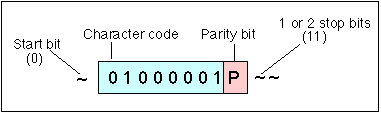
\includegraphics[width=0.4\textwidth]{gambar/parity.png}

  % Ubah sesuai dengan keterangan gambar yang diinginkan.
  \caption{Struktur parity bit}
  \label{fig:parityexample}
\end{figure}

% Contoh pembuatan tabel.
\begin{table}
  \caption{Contoh bit paritas}
  \label{tab:parityexample}
  \centering
  \rowcolors{3}{green!80!yellow!50}{green!70!yellow!40}
  \begin{tabular}{cccc}
    \toprule
    & & \multicolumn{2}{c}{8 bits including parity} \\
    7 bits of data & Count of 1 bits & even & odd \\
    \midrule
    0000000        & 0               & 00000000 & 00000001 \\
    1010001        & 3               & 10100011 & 10100010 \\
    1101001        & 4               & 11010010 & 11010011 \\
    1111111        & 7               & 11111111 & 11111110 \\
    \bottomrule
  \end{tabular}
\end{table}

Apabila sebuah string yang berisi bit-bit paritas ditransmisikan secara tidak benar atau korup, maka bit paritasnya akan salah. Hal tersebut mengindikasikan terjadinya \emph{parity error} saat transmisi. Bit paritas ini hanya bisa mendeteksi adanya error; tidak dapat melakukan koreksi error pada file yang terjadi, karena tidak ada mekanisme yang memungkinkan bit paritas untuk mengetahui bit yang mana yang korup. Lalu apabila meninjau Tabel \ref{tab:parityexample}, dapat diketahui bahwa bit paritas ini memiliki kelemahan. Bit paritas hanya mengecek jumlah bit ganjil atau genap tanpa meninjau jumlah asli bitnya. Hal ini mengakibatkan terjadinya kegagalan dalam menangkap error pada data. Sebagai contoh, jika A ingin mengirim data \verb|1001| dengan paritas genap maka bit paritasnya adalah \verb|0| sehingga yang ditransmisikan ke B adalah \verb|10010|. Terjadi error pada transmisi, sehingga yang sampai ke B adalah \verb|11011|. Akan tetapi, B menghitung jumlah bit dan mendapati genap, sehingga B akan menganggap data tersebut benar walaupun sebenarnya salah.

% Contoh input potongan kode dari file.
\lstinputlisting[
  language=Python,
  caption={Program perhitungan bit paritas genap.},
  label={lst:paritasgenap}
]{program/paritas_genap.py}

\begin{lstlisting}[
  language=Python,
  caption={Program perhitungan bit paritas ganjil},
  label={lst:paritasganjil}
]
def odd_parity(x):
    parity = 1
    while x:
        parity ^= x & 1
        x >>= 1
    return parity
\end{lstlisting}

Potongan kode pada Listing \ref{lst:paritasgenap} diatas adalah contoh kode yang berfungsi menemukan bit paritas genap. Untuk bit paritas ganjil tinggal mengganti inisialisasi variabel parity menjadi 1. Inputnya adalah \emph{integer} yang bisa kita jadikan biner dulu, seperti \verb|0b10001|.

% % Contoh pembuatan persamaan ilmiah.
% \begin{equation}
%   \label{eq:hukumpertama}
%   \sum \mathbf{F} = 0\; \Leftrightarrow\; \frac{\mathrm{d} \mathbf{v} }{\mathrm{d}t} = 0.
% \end{equation}

  % Ubah judul dan label berikut sesuai dengan yang diinginkan.
\section{Checksum}
\label{sec:checksum}

% Ubah paragraf-paragraf pada bagian ini sesuai dengan yang diinginkan.

Sebuah checksum merupakan suatu blok data berukuran kecil yang diperoleh dari blok data digital yang lainnya. Checksum memiliki tujuan untuk mendeteksi error yang mungkin saja terjadi ketika melakukan transmisi data pada memori maupun internet. Checksum biasanya digunakan untuk verifikasi \emph{integrity} dari sebuah data, dengan kata lain apakah datanya sudah dimodifikasi setelah checksum dibuat. Output dari sebuah algoritma fungsi \emph{hash cryptographic}, yang biasa disebut \emph{hashes} atau \emph{digest} digunakan sebagai checksum. Checksum biasanya direpresentasikan dengan menggunakan string hexadecimal (e.g., 69fac420b...), ukurannya berkisar antara 32 sampai 128 digit. Fungsi \emph{hash cryptographic} ini memiliki tiga properti utama, yakni pre-image resistance, second pre-image resistance, dan collision resistance \citep{bart1994}. Fungsi \emph{hash cryptographic} yang sering digunakan adalah MD5, SHA-1, dan SHA-2. MD5 merupakan salah satu fungsi \emph{hash cryptographic} pertama yang dicanangkan. Namun pada akhir 1990an, algoritma tersebut mulai ditinggalkan karena berhasil dirusak sehingga tidak baik untuk keamanan. SHA-1 direkomendasikan oleh National Institute of Standards and Technology (NIST) sampai pada tahun 2015, algoritmanya terbobol. Sekarang, SHA-2 menjadi algoritma terpopuler yang direkomendasikan NIST untuk melakukan verifikasi integritas file \citep{nistpolicy}.

\subsection{MD5}
\label{subsec:MD5}

Sebuah \emph{MD5 message-digest algorithm} adalah hash function yang \emph{cryptographically broken} tapi masih sering digunakan untuk membuat nilai hash 128 bit. \emph{Cryptographically broken} maksudnya adalah secara security sudah tidak aman atau \emph{vulnerable}. Pada awalnya, MD5 didesain sebagai fungsi \emph{hash cryptographic}, namun ditemukan banyak vulnerability pada MD5, yang membuat algoritma ini ditinggalkan. MD5 masih bisa digunakan untuk melakukan verifikasi integritas data, namun hanya untuk mengecek kerusakan data yang tidak disengaja. MD5 masih cocok digunakan untuk hal-hal non kriptografik, seperti menentukan partisi dari kunci tertentu pada database yang sudah dipartisi, dan juga beberapa orang masih memilih menggunakan MD5 daripada \emph{Secure Hash Algorithm} (SHA) karena beban komputasi yang lebih ringan \citep{martin2017}. MD5 didesain oleh Ronald Rivest tahun 1991 untuk menggantikan MD4, dan dispesifikasikan pada tahun 1992 sebagai RFC 1321. Salah satu kebutuhan dasar dari fungsi \emph{hash cryptographic} adalah harus secara komputasional tidak mungkin ditemukan dua buah data yang berbeda dan memiliki nilai hash yang sama. MD5 gagal melakukan hal tersebut dan berdampak cukup fatal. Pada tahun 2019, MD5 tetaplah secara luas digunakan, meskipun kelemahan yang dimiliki sudah banyak didokumentasikan oleh para ahli security \citep{md5vuln}. Sebuah \emph{collision attack} dengan menggunakan komputer 2.6 GHz Pentium 4 dapat menemukan collision pada MD5 dalam hitungan detik. MD5 menggunakan \emph{Merkle–Damgård construction}, jadi jika dua prefix dengan hash yang sama dapat dibuat, maka suffix umum dapat ditambahkan pada keduanya untuk membuat collision yang terjadi dapat diterima dan dianggap valid pada aplikasi yang menggunakannya.

MD5 digest sudah digunakan secara luas pada dunia perangkat lunak untuk memberikan sebuah jaminan dimana file yang ditransmisikan telah tiba dan datanya sama dengan data yang asli. Sebagai contoh, file pada server-server umumnya menyediakan MD5sum yang sudah dikomputasi untuk file tertentu, sehingga user yang mengunduh file tersebut dapat membandingkan apakah file yang diterima sama dan utuh dengan file asli yang terdapat pada server. Kebanyakan UNIX-based system menggunakan MD5sum pada package managernya. ROM pada Android juga menggunakan checksum jenis MD5 ini. MD5 juga biasa digunakan untuk hashing password satu arah, namun NIST tidak merekomendasikan MD5 untuk keperluan ini

\begin{figure} [ht]
  \centering
  % Ubah sesuai dengan nama file gambar dan ukuran yang akan digunakan.
  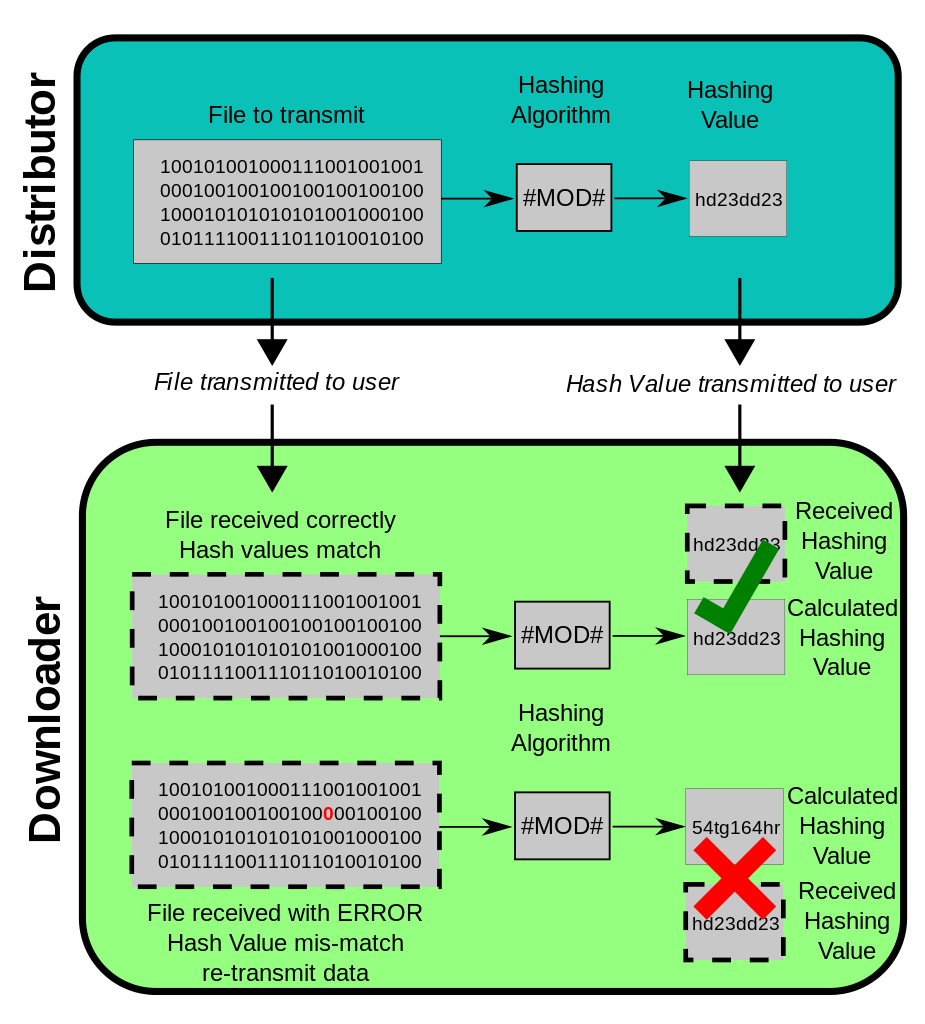
\includegraphics[width=0.4\textwidth]{gambar/hashing-file-transmission.png}

  % Ubah sesuai dengan keterangan gambar yang diinginkan.
  \caption{File transmisi dengan hashing}
  \label{fig:hashingfiletransmission}
\end{figure}

MD5 akan memproses pesan yang memiliki panjang bervariasi menjadi output dengan panjang 128 bit. Pesan masukan dipecah menjadi block-block 512 bit, dan pada pesan dilakukan padding agar panjangnya dapat dibagi dengan 512. Cara paddingnya adalah: pertama, satu bit, 1 ditambah pada akhir pesan. Kemudian bit ini diikuti dengan nol sebanyak yang dibutuhkan untuk membuat panjang message kurang dari 64 bit dari kelipatan 512. Bit sisa yang panjangnya 64 bit diisi dengan 64 bit yang merepresentasikan panjang pesan mulanya, modulo 2.

Algoritma inti dari MD5 bekerja pada keadaan 128-bit, dibagi menjadi 32-bit words, dinotasikan dengan \(A, B, C\), dan \(D\). Variabel tersebut diinisialisasi ke konstanta tertentu. Algoritma inti akan menggunakan tiap blok pesan berukuran 512-bit untuk memodifikasi statenya. Pemrosessan dari blok pesan terdiri dari 4 tahap, termed rounds; tiap tahap terdiri dari 16 operasi yang mirip berdasarkan fungsi linear \(F\), penjumlahan modular, dan rotasi ke kiri. Berikut persamaannya. Terdapat 4 fungsi yang mungkin terjadi, fungsi berbeda digunakan untuk tiap tahapan atau round.

\begin{equation}
\label{eq:md5sum}
F(B,C,D) = (B \land C) \lor (\neg B \lor D)
\end{equation}
\begin{equation}
G(B,C,D) = (B \land D) \lor (B \lor \neg D)
\end{equation}
\begin{equation}
H(B,C,D) = B \oplus C \oplus D
\end{equation}
\begin{equation}
I(B,C,D) = C \oplus (B \lor \neg D)
\end{equation}

% Contoh input potongan kode dari file.
\lstinputlisting[
  language=Python,
  caption={Program python sederhana untuk cek md5sum},
  label={lst:md5sum}
]{program/md5sum.py}

Pada Listing \ref{lst:md5sum} adalah contoh program python sederhana untuk melakukan checksum menggunakan MD5. Program tersebut menggunakan library bawaan bernama hashlib.

\subsection{SHA-1}
\label{subsec:SHA1}

SHA-1 merupakan fungsi \emph{hash cryptographic} yang menerima input lalu akan mengeluarkan output 160-bit (20 byte) nilai hash yang dikenal sebagai \emph{message digest}, yang biasanya adalah angka hexadesimal dengan panjang 40 digit. SHA-1 dibuat oleh NSA, badan keamanan Amerika. Sejak tahun 2005, SHA sudah tidak dianggap aman oleh badan-badan keamanan \citep{schneier2005}. NIST secara formal tidak memperbolehkan penggunaan SHA pada tahun 2013. Penggantian SHA-1 terbilang urgent pada penggunaannya dalam digital signature seperti SSL certificate. Semua web browser populer tidak menerima sertifikat SSL SHA-1 pada tahun 2017 \citep{mozilla2019,google2015}. SHA-1 memproduksi message digest dan prinsipnya mirip dengan MD5, namun membuat nilai hash yang lebih besar (160 bit vs 128 bit). Version control system seperti Git, Mercurial, dan Monotone menggunakan SHA-1 bukan untuk sekuriti, namun untuk pengecekan revisi dan untuk menjamin datanya tidak berubah karena korup yang tidak disengaja.

Untuk hash function yang mana \(L\) adalah jumlah bit di message digest, menemukan message yang sesuai dengan message digest dapat selalu dilakukan dengan metode \emph{brute force} yang kira-kira dilakukan \(2^L\) iterasi. Ini dinamakan preimage attack dan mungkin bekerja mungkin juga tidak tergantung dari \(L\) dan kekuatan komputasi dari komputer. Akan tetapi, sebuah \emph{collision}, yang terdiri dari menemukan dua pesan berbeda yang menghasilkan message digest yang sama memerlukan kurang lebih \(1.2\times{2^{L/2}}\) iterasi apabila menggunakan birthday attack. Beberapa aplikasi yang menggunakan cryptographic hashes, seperti penyimpanan password, tidak terlalu terdampak oleh collision attack. Membuat password yang bekerja untuk suatu akun membutuhkan preimage attack, dan juga akses ke hash pada password originalnya. Pada kasus tanda tangan dokumen, attacker tidak dapat langsung memalsukan signature dari dokumen yang sudah ada. Attacker harus membuat sepasang dokumen, satu yang tidak merusak, dan satu untuk merusak, dan membuat pemegang \emph{private key} untuk menandatangani dokumen yang tidak merusak.

\lstinputlisting[
  language=Python,
  caption={Program python sederhana untuk cek sha1sum},
  label={lst:sha1sum}
]{program/sha1.py}

Pada Listing \ref{lst:sha1sum} adalah contoh program python sederhana untuk melakukan checksum menggunakan algoritma SHA-1. Program tersebut menggunakan library bawaan bernama hashlib.

\subsection{SHA-2}
\label{subsec:SHA2}

SHA-2 merupakan perubahan yang cukup signifikan dibandingkan pendahulunya, SHA-1. SHA-2 family terdiri atas enam buah hash function dengan digests (nilai hash) yang bernilai 2254, 256, 384 atau 512 bit: SHA-224, SHA-256, SHA-384, SHA-512, SHA-512/224, SHA-512/256. Hash function pada SHA-2 digunakan secara luas pada sejumlah aplikasi dan protokol sekuriti seperti TLS dan SSL, PGP, SSH, S/MIME dan IPsec. SHA-256 digunakan dalam proses autentikasi package software di OS Debian. SHA-256 dan SHA-512 direncanakan untuk digunakan pada DNSSEC \citep{rfc5702}. Makin besar nilai hashnya maka artinya semakin aman dan sulit untuk menemukan collision, tetapi membutuhkan beban komputasi yang lebih tinggi.

\subsection{SHA-3}
\label{subsec:SHA3}

SHA-3 merupakan member terbaru dari family Secure Hash Algorithm (SHA), yang dirilis oleh NIST pada tahun 2015. Meskipun masih satu family, SHA-3 secara internal berbeda dengan SHA-1 dan SHA-2 yang strukturnya seperti MD5. SHA-3 merupakan subset dari \emph{Keccak} \citep{nist2012}. 

Keccak didasari dari pendekatan baru yang dinamakan sponge construction. Sponge construction didasari dari fungsi random atau fungsi permutasi, dan menerima (atau "menyerap", dalam istilah sponge) input data sebanyak apapun, kemudian mengoutput ("memeras") berapapun jumlah datanya, sambil bertindak sebagai \emph{pseudorandom function}. Pada state absorbing, blok pesan di-XOR menjadi subset dari state, yang kemudian ditransformasikan secara keseluruhan menggunakan fungsi permutasi \(f\). Pada state "squeeze", blok-blok output dibaca dari subset yang sama dari state, berselang-seling dengan fungsi transformasi state \(f\). Ukuran dari bagian pada state yang tertulis dan dibaca dinamakan "rate" (dinotasikan sebagai \(r\)), dan ukuran dari bagian yang tidak tersentuh oleh input/output dinamakan capacity (dinotasikan sebagai \(c\)). Kapasitas ini menentukan tingkat dari sekuritinya. Level maksimum dari sekuritinya adalah separuh dari kapasitasnya. Akgoritma dari \emph{Keccak} adalah sebagai berikut \citep{arshad2014}.

Fungsi theta terdiri dari tiga persamaan yang melibatkan operasi XOR sederhana dan bitwise cyclic shift.

\begin{equation}
  \label{eq:cx}
  C[X] = XOR(A[X,0], A[X,1], A[X,2], A[X,3], A[X,4])
\end{equation}

\emph{Circular shift} ke kiri pertama diaktifkan di lima jalur output. Setelah tahap ini, jalur terakhir menjadi yang pertama dan jalur kedua terakhir akan menjadi jalur terakhir. Kemudian circular shift ke kanan dilakukan pada lajur tersebut sehingga jalur pertama menjadi jalur terakhir dan jalur kedua menjadi jalur pertama. Sekarang circular shift ke kiri diterapkan pada setiap jalur untuk mengubah posisi dari bit pada tiap lajur \citep{arshad2014,chandran2016}.

\begin{equation}
  \label{eq:dx}
  D[X] = ROT(C[X - 1], C[X + 1, 1])
\end{equation}

Input state matrix dan output jalur yang didapat dari (\ref{eq:cx})(\ref{eq:dx}) di-XOR kan.

\begin{equation}
  \label{eq:axy}
  A[X,Y] = XOR(A[X,Y], D[X]), 0\leq X;Y\leq 4
\end{equation}

Rho (\(\rho\)) dan Pi (\(\Pi\)) dapat diekspresikan untuk menghitung array B berukuran 5\(\times\)5 dari state array A. Operasi dari rho dan Pi, melakukan rotasi sirkular sebanyak nilai tetap yang bergantun pada koordinat \(X\) dan \(Y\).

\begin{equation}
  \label{eq:rxy}
  r[X,Y], B[Y,2X+3Y] = ROT(A[X,Y], r[X,Y])
\end{equation}

Jalur yang dirotasikan ditempatkan di array B. Ini disebut sebagai Pi step. Indeks yang diambil adalah modulo 5.

Jalurnya dioperasikan dengan fungsi chi (\(\chi\)) seperti berikut.

\begin{equation}
  \label{eq:chi}
  A[X,Y]=B[X,Y]((\neg B[X+1,Y]) \land B[X+2,Y])
\end{equation}

Step Iota (\ref{eq:iota}) adalah step paling sederhana dari algoritma Keccak. Step ini hanya melakukan operasi XOR pada konstanta bit RC dengan jalur pada lokasi \([0, 0]\) dari matrix state baru A.

\begin{equation}
  \label{eq:iota}
  A[0,0]=XOR(A[0,0], RC)
\end{equation}

\lstinputlisting[
  language=Python,
  caption={Program python sederhana untuk cek sha3sum 512 bit},
  label={lst:sha3sum}
]{program/sha3.py}

Program yang ada di listing \ref{lst:sha3sum} menunjukkan program python sederhana untuk melakukan pengecekan file integrity menggunakan algoritma SHA-3 512-bit.

% % Contoh pembuatan tabel.
% \begin{table}
%   \caption{Contoh tabel sederhana}
%   \label{tab:tabelsederhana}
%   \centering
%   \begin{tabular}{lll}
%     \toprule
%     Heading1 & Heading2 & Heading3  \\
%     \midrule
%     One      & Two      & Three     \\
%     Four     & Five     & Six       \\
%     \bottomrule
%   \end{tabular}
% \end{table}

\lipsum[12]

% % Contoh pembuatan daftar.
% \begin{enumerate}
%   \item \lipsum[13][1-4]
%   \item \lipsum[13][5-8]
%   \item \lipsum[13][9-12]
% \end{enumerate}

  % Ubah judul dan label berikut sesuai dengan yang diinginkan.
\section{Cyclic Redundancy Check}
\label{sec:crc}

% Ubah paragraf-paragraf pada bagian ini sesuai dengan yang diinginkan.

% % Contoh input beberapa gambar pada halaman.
% \begin{figure*}
%   \centering
%   \subfloat[Hasil A]{\includegraphics[width=.4\textwidth]{example-image-a}
%     \label{fig:hasila}}
%   \hfil
%   \subfloat[Hasil B]{\includegraphics[width=.4\textwidth]{example-image-b}
%     \label{fig:hasilb}}
%   \caption{Contoh input beberapa gambar.}
%   \label{fig:hasil}
% \end{figure*}

Sebuah \emph{Cyclic Redundancy Check} adalah \emph{error-detecting code} yang biasa digunakan pada jaringan digital dan storage untuk mendeteksi adanya perubahan yang tidak diinginkan pada data. Blok data yang memasuki sistem CRC akan diberikan \emph{check value}, berdasarkan sisa dari pembagian polinomial dari kontennya. Saat pengambilan data, kalkulasi tersebut diulang lagi dan apabila check value tidak sesuai maka dapat dilakukan koreksi untuk menghindari data yang korup. CRC dapat digunakan untuk \emph{error-correction} \citep{dobbs2003}. Varian CRC-1 dikenal juga sebagai parity bit (\ref{sec:paritybit}).

Sejatinya, CRC merupakan tipe dari checksum, dan memiliki konsep yang mirip dengan checksum. Akan tetapi, terdapat perbedaan diantaranya sehingga saya memutuskan untuk memberikannya bab tersendiri. CRC merupakan checksum yang secara spesifik adalah \emph{position dependent checksum algorithm}. Dari namanya tersebut, CRC dapat mendeteksi perpindahan posisi, yang membuatnya menjadi integrity check yang umum digunakan. CRC juga populer dikarenakan kesederhanaannya dibandingkan algoritma checksum yang lainnya seperti MD5 dan SHA family. CRC juga lebih mudah untuk dianalisis secara matematis dan baik untuk mendeteksi error yang umum terjadi dikarenakan oleh noise pada transmission channel. CRC sendiri tidak didesain dengan tujuan kriptografik, karena CRC dapat direverse sehingga untuk alasan keamanan lebih dianjurkan untuk menggunakan SHA-2. CRC biasa digunakan dalam hal untuk menyalin atau memindahkan file serta kompres dan dekompres file.

\subsection{Integritas Data}
\label{subsec:crcdataintegrity}

Seperti yang sudah disebutkan sebelumnya, CRC didesain secara spesifik untuk keperluan error-checking, dimana CRC akan mendeteksi kesalahan dengan beban komputasi yang jauh lebih ringan dibandingkan dengan Cryptographic Hash Function. Maka dari itu, CRC tidak cocok untuk melindungi dari modifikasi data yang disengaja. Yang pertama, karena tidak ada autentikasi, \emph{attacker} dapat memodifikasi pesan dan menghitung ulang CRCnya tanpa terdeteksi. Ketika disimpan bersama dengan data, baik CRC maupun Cryptographic Hash Function tidak melindungi dari perubahan data yang disengaja. Aplikasi yang memerlukan proteksi dari serangan tersebut harus menggunakan mekanisme autentikasi kriptografik, seperti \emph{message authentication codes} (MAC) atau \emph{digital signatures}. Yang kedua, tidak seperti MD5 maupun SHA, CRC dapat dengan mudah direverse, yang membuat CRC tidak cocok untuk digunakan sebagai \emph{digital signatures} \citep{martin2006}. Yang ketiga, CRC memiliki hubungan yang mirip dengan fungsi linear \citep{poncho2016}. 

\begin{equation}
  \label{eq:crc1}
  CRC(x\oplus y) = CRC(x) \oplus CRC(y) \oplus c
\end{equation}

Dimana \(c\) bergantung dari panjang \(x\) dan \(y\). Persamaan \ref{eq:crc1} juga bisa dituliskan seperti berikut, dimana \(x\), \(y\), dan \(z\) memiliki panjang yang sama.

\begin{equation}
  \label{eq:crc2}
  CRC(x\oplus y \oplus z) = CRC(x) \oplus CRC(y) \oplus CRC(z)
\end{equation}

Maka, bahkan ketika CRC dienkripsi dengan \emph{stream cipher} yang menggunakan XOR sebagai operasi kombinasinya, baik pesan maupun CRC dapat dimanipulasi tanpa sepengetahuan dari \emph{encryption key}, ini merupakan salah satu \emph{design flaws} dari protokol Wired Equivalent Privacy (WEP) \citep{winget2003}.

\subsection{Algoritma}
\label{subsec:crcalgorithm}

Komputasi dari CRC diturunkan dari polynomial division, modulo dua. Ini menyerupai pembagian dari pesan string biner, dengan nol bit yang jumlahnya tetap diappend oleh string "generator polynomial", tetapi dengan menggunakan XOR, bukan pengurangan. Pembagian jenis ini sudah direalisasikan di harware dengan shift register yang sudah dimodifikasi \citep{dubrova2012}. Contoh dari implementasi polynomial division pada hardware, misalnya kita mencoba untuk menghitung CRC 8-bit dari pesan 8-bit yang terdiri dari karakter ASCII "W", yang binernya adalah \(01010111_2\), desimal \(87_10\) atau hexadecimal \(57_16\). Sebagai ilustrasi, kita menggunakan CRC-8-ATM (HEC) polinomial \(x^6+x^2+x+1\). Menuliskan bit pertama yang ditransmisikan (koefisien dari pangkat tertinggi \(x\)) di sebelah kiri, sesuai dengan string 9-bit "100000111". Nilai byte \(57_16\) dapat dikirimkan dalam dua urutan berbeda, bergantung dari konvensi urutan bit yang digunakan. Tiap urutan menghasilkan pesan polinomial \(M(x)\) yang berbeda. Msbit-first, \(x^6+x^4+x^2+x+1\) = 01010111, bila lsbit-first, \(x^7+x^6+x^5+3+1\) = 11101010. Nilai ini dapat dikalikan dengan \(x^8\) untuk menghasilkan dua pesan 16-bit polinomial \(x^8M(x)\). Menghitung sisanya terdiri dari mengurangi kelipatan dari generator polinomial \(G(x)\). Ini hanya seperti pembagian desimal, tapi lebih sederhana karena kelipatan yang mungkin hanyalah 0 dan 1, dan pengurangannya meminjam dari "tak terhingga", bukan mengurangi dari digit yang lebih tinggi. Karena kita tidak peduli dengan hasil bagi, maka tidak perlu dituliskan.

\begin{figure} [ht]
  \centering
  % Ubah sesuai dengan nama file gambar dan ukuran yang akan digunakan.
  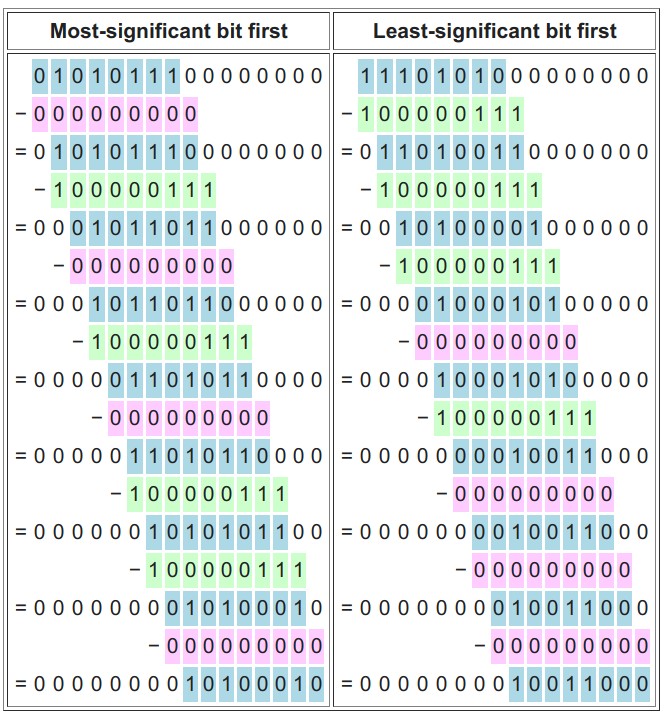
\includegraphics[width=0.4\textwidth]{gambar/komputasicrc.png}

  % Ubah sesuai dengan keterangan gambar yang diinginkan.
  \caption{Perhitungan polynomial division}
  \label{fig:crccomputation}
\end{figure}

Perhatikan bahwa untuk setiap pengurangan, bit-bitnya dibagi menjadi 3 bagian, grup yang berisi nol, grup yang tidak diubah dari originalnya, dan grup yang berwarna biru, yang "menarik". Grup yang menarik ini panjangnya 8-bit, menyamai pangkat dari polinomial. Setiap langkah, kelipatan yang benar dikurangi untuk membuat grup nol menjadi satu bit lebih besar, dan grup yang tidak berubah menjadi satu bit lebih pendek, hingga akhirnya meninggalkan satu sisa.

% Contoh input potongan kode dari file.
\lstinputlisting[
  language=Python,
  caption={Program CRC.},
  label={lst:crccomputation}
]{program/crccomputation.py}

Program dari listing \ref{lst:crccomputation} berisi fungsi yang akan mereturn nilai sisa awal dari CRC untuk input dan polinomial yang ditentukan, entah dengan 1 atau 0 sebagai padding awalnya.

\begin{lstlisting}[
  language=Python,
  caption={Output dari listing \ref{lst:crccomputation}.},
  label={lst:outputcrc}
]
>>> crc_remainder('11010011101100', '1011', '0')
'100'
>>> crc_check('11010011101100', '1011', '100')
True
\end{lstlisting}

\lstinputlisting[
  language=C,
  caption={Program CRC dalam bahasa C.},
  label={lst:crcwithc}
]{program/crc.c}

Listing \ref{lst:crcwithc} merupakan algoritma CRC-32 \citep{microsoft2019} dalam bahasa C. Variable \lstinline{CRCTable} adalah memoization dari kalkulasi yang harus diulang untuk setiap byte dari pesan.

\subsection{Kompresi Data}
\label{subsec:kompresidata}

CRC digunakan untuk melakukan kalkulasi dari semua data yang ada di dalam file yang terkompresi. Nilai CRC akan dikalkulasi setiap kali ada file baru yang ditambahkan kedalam archive. Ketika archive atau file terkompresi di dekompresi, maka program akan mengkalkulasi nilai CRC kembali dan membandingkannya dengan yang ada di archive. Apabila terdapat perbedaan pada CRC value, maka biasanya akan ditampilkan pesan CRC error, yang mengindikasikan bahwa file yang terekstrak tidak sama dengan file yang awalnya dikompresi. Hal ini biasanya terjadi ketika file yang dikompresi didalam archive rusak. Hal ini juga dapat terjadi walaupun hanya satu file didalam archive yang korup.

Nilai dari CRC itu sendiri tidak mengatakan bahwa file anda korup atau tidak. Maka, ketika kita mengecek metadata dari archive atau mengkompresi file dan menemukan nilai CRC-nya, bukan berarti archive kita telah rusak. Hal tersebut hanya menunjukkan nilai awal dari CRC file yang terkompresi. Kebanyakan software untuk melakukan kompresi seperti 7zip dan WinRAR sudah memiliki mekanisme ini \citep{7zip}.

  % Ubah judul dan label berikut sesuai dengan yang diinginkan.
\section{Kesimpulan}
\label{sec:kesimpulan}

% Ubah paragraf-paragraf pada bagian ini sesuai dengan yang diinginkan.

Dari semua bagian yang sudah diberikan pembahasannya pada makalah ini, dapat diberi kesimpulan sebagai berikut. Parity Bit adalah salah satu cara untuk melakukan uji integritas file yang paling sederhana, tetapi pada penggunaannya terdapat kelemahan-kelemahan seperti jumlah bit yang sama-sama genap maupun ganjil tetapi berbeda dari yang aslinya akan dianggap tidak benar. Parity bit sendiri memiliki kelebihan seperti tidak memerlukan beban komputasi yang besar. Checksum sendiri merupakan istilah yang lebih luas dari algoritma-algoritma yang digunakan untuk melakukan pengecekan integritas. Terdapat banyak algoritma untuk melakukan checksum, salah satunya yang populer adalah MD5. MD5 merupakan algoritma hash function yang umum digunakan, meski sekarang hanya digunakan untuk sekedar melakukan cek integritas pada file yang tidak dimodifikasi secara sengaja. Hal ini terjadi karena komputer sekarang makin cepat sehingga metode brute force untuk menemukan collision dapat dengan mudah dilakukan. MD5 adalah varian dari message digest algorithm. SHA-1 merupakan generasi kedua dari keluarga SHA (Secure Hash Algorithm). SHA-1 juga sudah ditinggalkan karena alasan keamanan yang sama dengan MD5. SHA-2 merupakan hash function algorithm yang paling umum digunakan sekarang. NIST masih merekomendasikan SHA-2, namun disarankan menggunakan hash value yang besar agar semakin aman. SHA-2 juga dapat digunakan untuk melakukan pengecekan integritas file, namun apabila tidak memedulikan aspek sekuriti tidak disarankan karena beban komputasi yang lebih tinggi. SHA-3 merupakan terobosan terbaru dari keluarga SHA, karena menggunakan pendekatan yang berbeda dari varian sebelumnya, Keccak Algorithm. SHA-3 diyakini lebih aman dalam masalah anti collision, namun belum secara luas digunakan. CRC atau Cyclic Redundancy Check merupakan salah satu jenis checksum namun tidak diperuntukkan untuk keamanan. CRC bagus digunakan untuk melakukan verifikasi saat menyalin file ataupun pengarsipan file. Algoritma yang digunakan CRC juga terbilang tidak serumit MD5 dan SHA, sehingga pada \emph{Integrated Ciruit} biasanya sudah diaplikasikan dan siap digunakan. 


  % Menyeimbangkan bagian akhir di kedua kolom
  \balance

  % Menampilkan daftar pustaka dengan format IEEE
  \bibliographystyle{IEEEtranN}
  \bibliography{pustaka/pustaka.bib}

\end{document}
